% Template from https://www.overleaf.com/latex/templates/ieee-conference-template/grfzhhncsfqn
\documentclass[conference]{IEEEtran}
\IEEEoverridecommandlockouts
% The preceding line is only needed to identify funding in the first footnote. If that is unneeded, please comment it out.
\usepackage{cite}
\usepackage{amsmath,amssymb,amsfonts}
\usepackage{algorithmic}
\usepackage{graphicx}
\usepackage{textcomp}
\usepackage{xcolor}
\def\BibTeX{{\rm B\kern-.05em{\sc i\kern-.025em b}\kern-.08em
    T\kern-.1667em\lower.7ex\hbox{E}\kern-.125emX}}
\begin{document}

% From: https://tex.stackexchange.com/a/458208
\makeatletter
\newcommand{\linebreakand}{%
  \end{@IEEEauthorhalign}
  \hfill\mbox{}\par
  \mbox{}\hfill\begin{@IEEEauthorhalign}
}
\makeatother

\title{Vehicle-to-Vehicle (V2V) Communication Implementation\\
\thanks{University of Florida}
}

\author{
    \IEEEauthorblockN{Gunnar Fandrich}
    \IEEEauthorblockA{
        \textit{Group: Autogators} \\
        \textit{Electrical and Computer Engineering} \\
        \textit{University of Florida} \\
Gainesville, Florida \\
todo@ufl.edu
    }
    \and
    \IEEEauthorblockN{Mark Lai}
    \IEEEauthorblockA{
        \textit{Group: Autogators} \\
        \textit{Electrical and Computer Engineering} \\
        \textit{University of Florida} \\
Gainesville, Florida \\
todo@ufl.edu
    }
    \and
    \IEEEauthorblockN{Rafael Hernandez-Lopez}
    \IEEEauthorblockA{
        \textit{Group: Autogators} \\
        \textit{Electrical and Computer Engineering} \\
        \textit{University of Florida} \\
Gainesville, Florida \\
rhernandezlopez1@ufl.edu
    }
    \linebreakand
    \IEEEauthorblockN{Rohan Malik}
    \IEEEauthorblockA{
        \textit{Group: Autogators} \\
        \textit{Electrical and Computer Engineering} \\
        \textit{University of Florida} \\
Gainesville, Florida \\
todo@ufl.edu
    }
}

\maketitle

\begin{abstract}
Vehicle-to-vehicle (V2V) allows communication between vehicles, promoting driver
awareness and potentially reducing the number of collisions. Existing V2V
implementations (cellular vehicle-to-everything, C-V2X) rely on cloud data,
whereas the implementation shown in this paper does true V2V between vehicles. A
mockup utilizing two ESP32 with a time-of-flight (ToF) sensor and accelerometer
communicate using UDP to deliver a proof-of-concept for V2V that can be used as
a base for V2V.
\end{abstract}

\begin{IEEEkeywords}
V2V, vehicles, driver, awareness, C, ESP32, UDP
\end{IEEEkeywords}

\section{Introduction}
As society moves towards utilizing more autonomous driving systems, vehicles can
act as a network to promote efficient and safe driving. This network is referred
to as vehicle-to-vehicle (V2V). Automotive vehicles should communicate with each
other through V2V to increase driver awareness and reduce the number of
collisions.

The current state of V2V is nonexistent. The closest thing on the market to V2V
is the 2023 Safety Cloud for Chrysler Vehicles, which is implemented through a
cellular network to create C-V2X (cellular vehicle-to-everything) \cite{cv2x}.
While this is fairly close to V2V, passing through a cloud does not exhibit true
V2V. Ideally the cars would communicate directly to each other, which is what is
covered by the implementation discussed in this paper. Additionally, Stellantis
announced vehicle-to-grid (V2G) testing in 2019 \cite{v2g}.

In 1999, the FCC designated a 75 MHz spectrum in the 5.9 GHz band for dedicated
short-range communications (DSRC) \cite{fcc_band}. Unfortunately, this band was
reallocated in 2020 for unlicensed WiFi use due to the failure of automobile
makers to release V2X production cars. Due to the removal of this band, we chose
UDP over WiFi as an acceptable simplified protocol for V2V. Ideally, UDP would
be replaced with another protocol built on top of UDP, or similar protocol,
specifically for V2V and operate on an FCC-designated band for V2V.

V2V will be illustrated using an ESP32 paired with time-of-flight (ToF) sensor
and accelerometer. Each ESP32 represents a simplified car, and communicate with
each other using UDP. UDP was chosen as the protocol to allow ad hoc car
networks to be formed as well as allow dropped packets once a car leaves the
network.

\section{V2V implementation}
This section covers our V2V implementation, the features and the mockup.

\subsection{Features}

\subsection{Hardware Mockup}

\section{Results}

\paragraph{LTH Mand} After low-temperature hydrogenation \cite{knekr}, the resist layer will
be etched and expose the SiARC underneath. This results in the stack from
Fig.~\ref{lth_mand}.
TODO: Explain what we use this for.

\begin{figure}[htbp]
\centerline{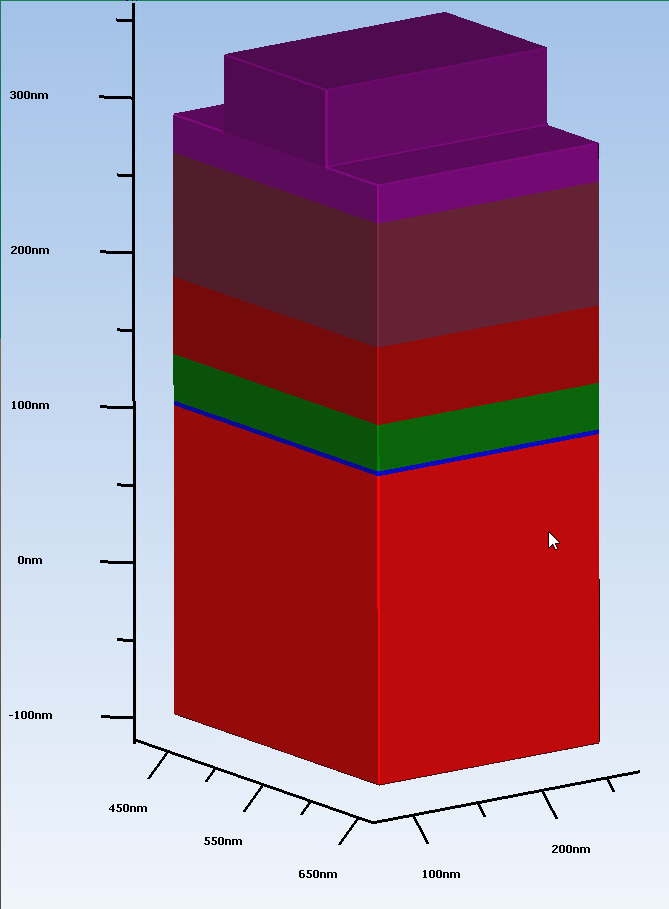
\includegraphics[width=\linewidth]{pics/lth_mand.png}}
\caption{The silicon stack after LTH Mand.}
\label{lth_mand}
\end{figure}

\paragraph{RIE Mand} Reactive ion etching (RIE) \cite{1481759} is used to cut
the SiARC layer, exposing the ODL underneath.

\section{Security}
Our implementation of V2V has room to improve. A V2V implementation usable on
the market would address a few security concerns.

\subsection{Packet Security}
As our UDP packets are being broadcasted to everyone in the nearby vecinity, an
attacker only needs to be located near the network to be considered a ``car''.
This means that anyone could send fake messages or tamper with existing packets.
This leaves room for improvement in terms of admitting ``cars'' on the network,
and properly identifying nodes on the network as ``car'', ``adversary'', or
``miscellaneuos'' nodes.

Attackers on the network could potentially leverage this limitation to inhibit
the flow of traffic by broadcasting that there is some blockade ahead (ToF
sensor data shows car ahead, accelerometer data shows there is no/little
movement). Attackers could also target individual vehicles with a similar idea.
They could send false packets to make the victim vehicle think it has to brake
suddenly, potentially crashing with vehicles behind them or causing them to
brake too fast. If the victim is carrying a heavy load, such as a large trailer,
braking too fast can compromise the stability of their vehicle and potentially
swerve out of control or unlatch their trailer.

\subsection{Network Security}
A member of the ad hoc network may be either callibrated to send too many
packets or is an attacker. In a case where the packet traffic is too heavy, a
denial of service attack (DoS) may occur. This should be addressed as well
before V2V is accepted by car manufacturers.

As the network is completely open to new ``cars'', attackers may be able to
probe the network for more vulnerabilities than those discussed. For example,
perhaps some UDP misconfiguration could be leveraged to forward UDP packet
contents to a CAN bus, or similar idea.

\section{Conclusion}
Lots of things happen in the 14 nm process flow.

\clearpage
\bibliographystyle{IEEEtran}
\bibliography{bibs}

\end{document}

